% !TEX program = lualatex
\documentclass[border=6pt]{standalone}
% ---------------------------------------------------------------------------
% tikzpreamble.tex -- shared by main.tex and by every standalone in tikz/
% ---------------------------------------------------------------------------
\usepackage{amsmath}
\usepackage{amssymb}
\usepackage{tikz}
\usepackage{circuitikz}
\usetikzlibrary{arrows.meta,calc,positioning,decorations.pathmorphing,decorations.pathreplacing,
                decorations.markings,patterns,angles,quotes,fit,
                shapes.geometric,shapes.misc,backgrounds,intersections}

\ctikzset{bipoles/length=0.85cm}
\ctikzset{resistors/scale=0.85}
\ctikzset{capacitors/scale=0.9}

\tikzset{
  wire/.style      = {line width=0.7pt},
  dashedwire/.style= {line width=0.7pt, densely dashed},
  term/.style      = {circle, draw, line width=0.6pt, fill=white,
                      inner sep=0pt, minimum size=4.5pt},
  node dot/.style  = {circle, fill=black, inner sep=0pt, minimum size=4pt},
  boxlabel/.style  = {font=\sffamily\small},
  annot/.style     = {font=\small, align=left},
  phasor/.style    = {-{Stealth[length=3.2mm,width=2.2mm]}, line width=1.1pt},
  thinphasor/.style= {-{Stealth[length=2.6mm,width=1.8mm]}, line width=0.7pt},
  axis line/.style = {-{Stealth[length=2.6mm,width=1.8mm]}, line width=0.6pt},
  guide/.style     = {densely dashed, line width=0.4pt, gray},
}
\usepackage{siunitx}

\begin{document}
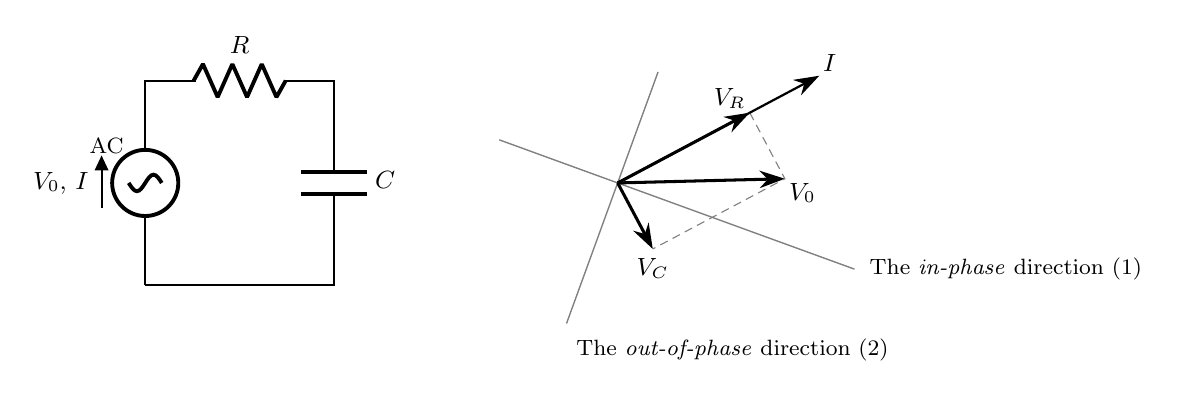
\begin{tikzpicture}[every node/.style={font=\small}]
  % ---- series RC circuit -------------------------------------------------
  \begin{scope}
    \draw[wire] (0,0) to[sV={$V_0,\,I$},invert] (0,2.6)
                      to[R=$R$] (2.4,2.6)
                      to[C=$C$] (2.4,0) -- (0,0);
    \node[font=\footnotesize,anchor=south east] at (-0.15,1.55) {AC};
  \end{scope}

  % ---- phasor diagram ----------------------------------------------------
  \begin{scope}[shift={(6.0,1.3)},rotate=-20]
    \draw[line width=0.5pt,gray] (-1.6,0) -- (3.2,0) coordinate (inph);
    \draw[line width=0.5pt,gray] (0,-1.9) -- (0,1.5) coordinate[at start] (outph);
  \end{scope}
  \node[anchor=west,font=\footnotesize] at ([xshift=2pt]inph)
      {The \textit{in-phase} direction (1)};
  \node[anchor=north west,font=\footnotesize] at ([yshift=-2pt]outph)
      {The \textit{out-of-phase} direction (2)};
  \begin{scope}[shift={(6.0,1.3)}]
    \coordinate (O) at (0,0);
    \coordinate (VR) at (28:1.9);
    \coordinate (VC) at (-62:0.95);
    \coordinate (V0) at ($(VR)+(VC)$);
    \draw[phasor] (O) -- (VR) node[anchor=south east,inner sep=1pt] {$V_R$};
    \draw[phasor] (O) -- (VC) node[anchor=north,inner sep=3pt] {$V_C$};
    \draw[phasor] (O) -- (V0) node[anchor=north west,inner sep=1pt] {$V_0$};
    \draw[guide] (VR) -- (V0) -- (VC);
    \draw[phasor,line width=0.8pt] (O) -- (28:2.9) node[anchor=south west,inner sep=1pt] {$I$};
  \end{scope}
\end{tikzpicture}
\end{document}
